\documentclass[12pt]{article}

\usepackage{sectsty}
\usepackage{fullpage}
\usepackage{graphicx}

\sectionfont{\large}
\begin{document}\vspace{0.5in}
\begin{center}\begin{large}\textbf{Raj Krishna Srivastava}\end{large}\end{center}\textbf{\hrulefill}\\

\begin{tabular}{@{}p{4in}p{3in}}
Room No-A7 & {Phone:}+91-9721377988 \\
Dr. S RadhaKrishnan Hostel & {E-mail:}krishna\_raj007@yahoo.in\\
University of Allahabad \\
Allahabad\\
& 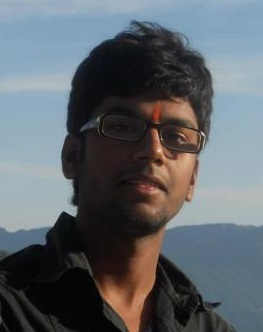
\includegraphics[scale=0.4]{rajKrishna.jpg}\\
\end{tabular}
\section*{Objective}
To develop my technical skills by working  and personality and can learn by itself; providing its users experience like never before.   
\section*{Education}
\begin{tabular}{|l|l|l|l|l|}
\hline
Degree & College/School & University & Passing Year & Pass Percentage\\
\hline
B. Tech & JK Institute of Applied Physics and Tchnology & Allahabad University & 2017 & 69.96 (till 5th sem)\\
\hline
Intermediate & City Montessori School & ICSE & 2013 & 95.80\\
\hline
High School & City Montessori School & ICSE & 2011 & 95.60\\
\hline
\end{tabular}

\section*{Projects}
\begin{itemize}
\item[$\bullet$]\textbf{Puzzle Solver Robot.}\\November 2015- Feb 2016\\Members: Keshav Bihani, G. HarshaVardhan, Shantam Srivastava

This project was based on OpenCv and Python and implemented on Atmega 2560. It used basic image processing technique to sense an image and then solve the puzzle using the input image.
\item[$\bullet$]\textbf{Online Examination Portal}\\May 2015- July 2015\\
The project was based on Jsp and used Javascript and Ajax. It is an online portal where examination with multiple choice answers can conducted.  
\item[$\bullet$]\textbf{Waste Segregating Robot.}\\October 2014-Jan 2015 \\Members: Keshav Bihani, G. HarshaVardhan, Shantam Srivastava

This project was based on Atmega 2560 to segregate waste based on its size and colour.It did win the second position in eYRC competition amongst 52 other teams that participated.
\end{itemize}
\section*{Training and Internships}
\begin{enumerate}
\item Advansed JAVA(Servlets and JSP).\\ May 2015- June 2015. Spectrum Technologies, Allahabad.
\item Core Java(J2SE).\\ December 2014- January 2015. Spectrum Technologies, Allahabad.
\item Embedded Systems.\\May 2014- July 2014. Labsguru Technologies, Lucknow.
\end{enumerate}
\end{document}